\chapter{Fundamentação teórica}

Este capitulo apresentada conceitos, técnicas e ferramentas relevantes ao desenvolvimento
do trabalho e à compreensão das próximas seções. O capítulo abrange fundamentos sobre arquitetura de \textit{software}, banco de dados e processo de desenvolvimento de \textit{software}.

\section{Arquitetura de \textit{software}}
\label{fundArquietura}

Sistemas grandes são sempre decompostos em subsistemas que fornecem algum conjunto de serviços relacionados. O processo inicial de projeto, que consiste em identificar esses subsistemas e estabelecer um \textit{framework} para o controle e a comunicação de subsistemas, é denominado projeto de arquitetura de software. \cite{sommerville}

A arquitetura de software; portanto, refere-se aos componentes de alto nível de um sistema de \textit{software} e à disciplina de criação destes. Cada um dos seus componentes incorpora elementos de \textit{software}, suas inter-relações e propriedades que os constituem. Além disso, define tarefas necessárias para serem realizadas pelas equipes que constituem o projeto.


\subsection{Arquitetura cliente-servidor}
\label{arquiteturaClienteServidor}

O modelo de arquitetura cliente-servidor é um modelo em que o sistema é organizado como um conjunto de serviços onde servidores e clientes associados os acessam e usam. Os clientes geralmente precisam saber nome e serviços disponíveis que os servidores oferecem. No entanto, servidores não precisam saber nomes nem quantos clientes existem. Essencialmente, um cliente faz um pedido a um servidor e espera até receber uma resposta \cite{pressman}. Exemplos de aplicativos de computador que usam o modelo cliente-servidor são \textit{e-mail}, impressão em rede e a Internet \cite{kurose}.


\subsection{Arquitetura centrada em dados}
\label{arquiteturaCentralizadaDados}

Arquitetura centrada em dados é um modelo de arquitetura de \textit{software} onde os bancos de dados são imprescindíveis para o funcionamento do sistema. Um sistema provido desta arquitetura processa solicitações de usuários a um banco de dados para diferentes tipos de ações como leitura ou escrita (inserir, atualizar ou remover) sobre os dados \cite{lewisBook}. A Figura \ref{dataCenteredArchitecture} exibe um estilo típico de arquitetura centrada em dados.

\begin{figure}[ht]
    \caption{Arquitetura centrada em dados: \textit{software} cliente acessa um repositório central independentemente de quaisquer alterações nos dados ou ações de outros clientes. }
       	\begin{center}
            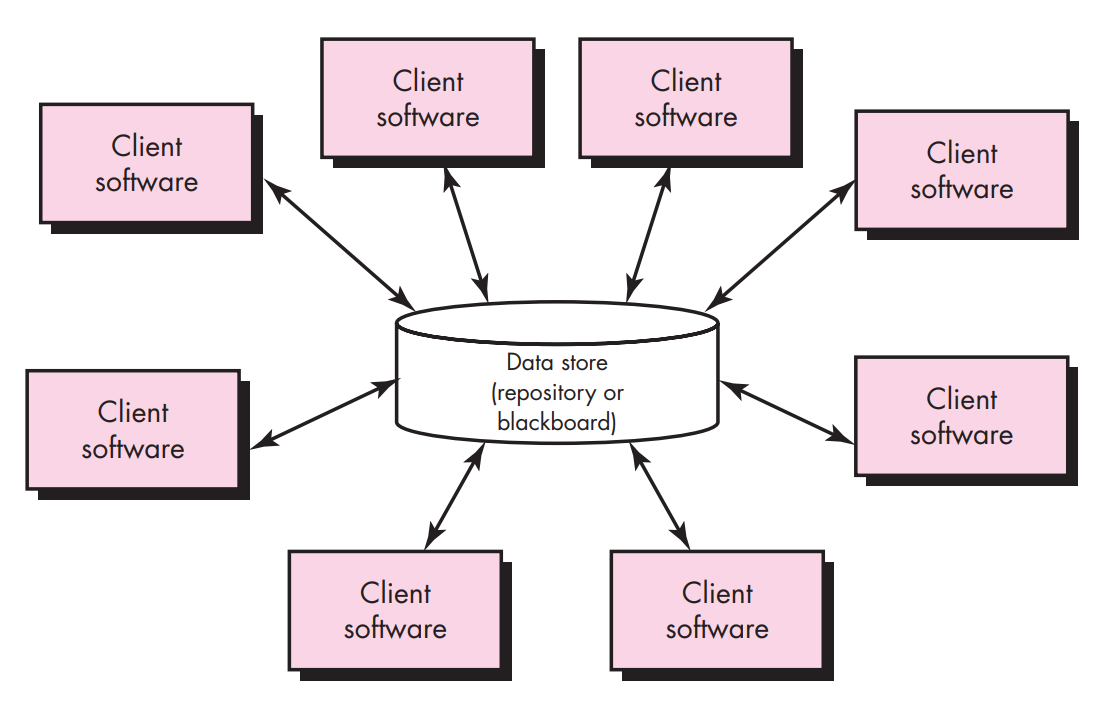
\includegraphics[width=0.75\textwidth]{arquitetura-centralizada-dados.png}
        \end{center}
    \label{dataCenteredArchitecture}
    \legend{\cite{pressman}}
\end{figure}


\subsection{Arquitetura MVC}
\label{arquiteturaMVC}

A arquitetura MVC, Modelo-visão-controlador, é um padrão arquitetural comumente usado para desenvolver interfaces de usuário que divide um aplicativo em três partes interconectadas: modelo, visão e controlador \cite{mvcCookbook}. Este padrão de arquitetura desacopla os três componentes principais, permitindo o reuso mais eficiente de código e desenvolvimento paralelo entre eles. 

O modelo engloba todo domínio específico à aplicação e seu processamento lógico como funcionalidades e acesso a dados externos e fontes de informação. A visão é responsável por exibir, na saída de dados, o conteúdo do modelo em um formato legível e requisitado pelo usuário final. O controlador, então, coordena a comunicação entre o modelo e a visão de acordo com as requisições do usuário. A Figura \ref{dataMVCArchitecture} ilustra a arquitetura MVC.

\begin{figure}[ht]
    \caption{Arquitetura MVC em aplicação \textit{web}.}
       	\begin{center}
            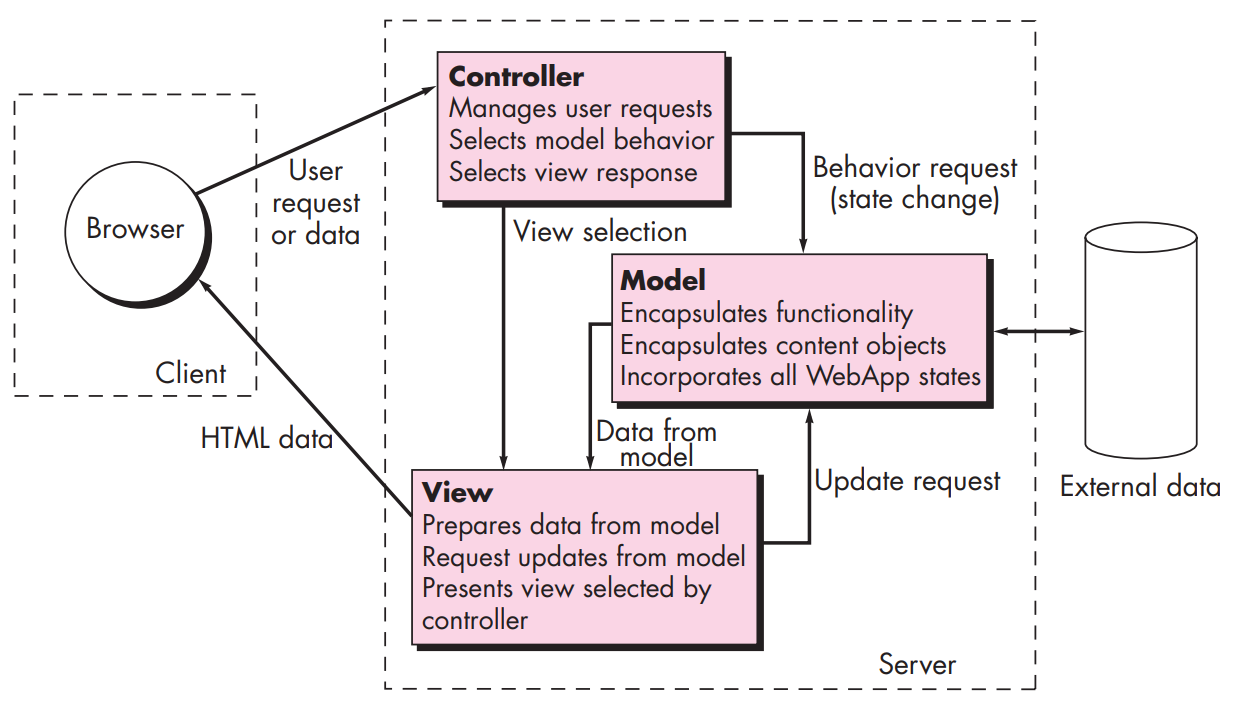
\includegraphics[width=0.75\textwidth]{arquitetura-mvc.png}
        \end{center}
    \label{dataMVCArchitecture}
    \legend{Fonte: \cite{pressman}}
\end{figure}


\section{Banco de dados}
\label{fundBD}

Um banco de dados pode ser definido como um conjunto de dados integrados que tem por objetivo atender a uma comunidade de usuários \cite{heuser}. Eles possuem uma coleção organizada de dados, geralmente armazenados e acessados por \textit{softwares} de computador. Devido aos avanços tecnológicos nessa área, bancos de dados foram aumentando sua complexidade e, para manter um sistema robusto, que incorpora funções de definição, alteração e recuperação de dados, são utilizados SGBDs.

Contudo, o processo de criação de um banco de dados para o \textit{software} de uma aplicação sugere a utilização de técnicas de construção de um projeto de banco de dados. No projeto, são considerados dois níveis de abstração de modelo de dados para sua implementação: o modelo conceitual e o modelo lógico.

\subsection{Modelo conceitual}
\label{fundBDModelagem}

A modelagem conceitual é utilizada para obter uma descrição abstrata, independente de implementação em computador, dos dados que serão armazenados no banco de dados. A técnica de modelagem de dados mais difundida e utilizada é a abordagem entidade-relacionamento (ER) \cite{heuser}. Através dela, os modelos de dados são representados graficamente por um diagrama entidade-relacionamento (DER) que captura necessidades da organização independente de implementação \cite{peterChen1976}. A Figura \ref{modelagemBDExemplol} apresenta um DER parcial presente na modelagem conceitual da rede social implementada.

\begin{figure}[h]
    \caption{Exemplo de modelagem conceitual.}
       	\begin{center}
            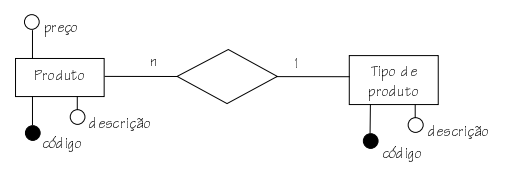
\includegraphics[width=0.68\textwidth]{figuras/modelo-conceitual.png}
        \end{center}
    \label{modelagemBDExemplol}
    \legend{Fonte: \cite{heuser}}
\end{figure}

\subsection{Modelo lógico}
\label{fundBDProjeto}

O projeto lógico consiste na transformação de um modelo ER em um modelo lógico. Este implementa de forma concreta, a nível de SGBD relacional, os dados representados no modelo ER.

Um determinado modelo ER pode ser implementado através de diversos modelos relacionais, que contém as informações especificadas pelo DER. Todos podem ser considerados uma implementação correta do modelo ER considerado. Entretanto, diferentes modelos relacionais podem resultar em diferentes performances do sistema construído sobre o banco de dados. 

No processo de transformação do modelo ER para o modelo relacional, foram utilizadas as seguintes regras de transformação \cite{heuser} a fim de obter uma melhor performance do sistema: 

\begin{itemize}
    \item Obter um banco de dados que permita boa performance de instruções de consulta e alteração do banco de dados.
    
    \item Obter um banco de dados que simplifique o desenvolvimento e a manutenção de aplicações.
    
    \item Evitar junções, ou seja, ter os dados necessários a uma consulta em uma única linha.
    
    \item Diminuir o número de chaves primárias.
    
    \item Evitar campos opcionais.
    
\end{itemize}

A Figura \ref{modelagemBDLogicoExemplol} apresenta a transformação do modelo ER para o modelo relacional do exemplo apresentado na figura \ref{modelagemBDExemplol}.

\begin{figure}[h]
    \caption{Exemplo de modelo lógico de tabelas em um SGBD.}
       	\begin{center}
            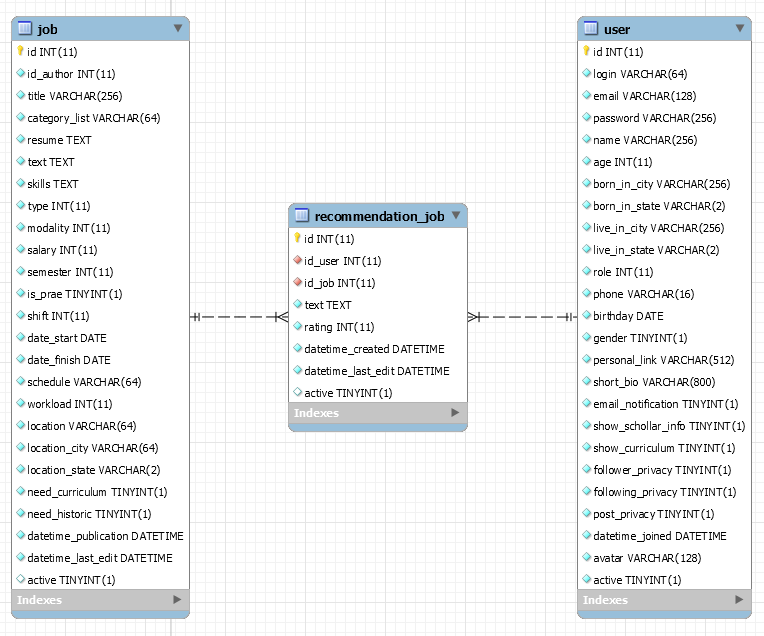
\includegraphics[width=0.75\textwidth]{figuras/er-exemplo.png}
        \end{center}
    \label{modelagemBDLogicoExemplol}
    \legend{Fonte: Autor}
\end{figure}

O banco de dados utilizado na rede social foi o SGBD relacional MySQL. A ferramenta é livre, popular, robusta e amplamente utilizada em aplicações na Internet \footnote{\url{https://db-engines.com/en/ranking} Acesso em outubro de 2018} \cite{mysql}. O MySQL utiliza a linguagem SQL, \textit{Structured Query Language}, padrão dos bancos de dados relacionais para realizar consultas e atualizar informações nos dados armazenados pelo sistema \cite{sqlCompleteBook}.

\section{Processo de desenvolvimento de \textit{software}}

A Engenharia de \textit{software} é um ramo da engenharia cujo foco é o desenvolvimento de sistemas de \textit{software} de alta qualidade dentro de custos adequados. Embora não existam limitações físicas em seu potencial, a falta de restrições naturais significa que o \textit{software} pode facilmente se tornar complexo e, portanto, de difícil compreensão \cite{sommerville}.

Para contornar tais problemas, uma das áreas de estudo da Engenharia de \textit{software} é a de processo de desenvolvimento de \textit{software}. Este é uma metodologia para as atividades, ações e tarefas necessárias para desenvolver um \textit{software} de alta qualidade. Pode-se considerar processo de \textit{software} também como o roteiro na elaboração de um produto ou sistema, pois segue uma série de passos previsíveis, apresenta qualidade e possui um prazo de entrega estabelecido \cite{pressman}.

Nesta seção é abordada a metodologia ágil e, posteriormente, o Scrum e Kanban, que são \textit{frameworks} de desenvolvimento de \textit{software} ágil. Ambos foram utilizados na implementação do protótipo deste trabalho.


\subsection{Metologia ágil}
\label{fundSWAgil}

A metodologia ágil é uma abordagem para o desenvolvimento de \textit{software} que prioriza o desenvolvimento do sistema à sua documentação e elaboração metódica no projeto. Geralmente conta com uma abordagem interativa para especificação, desenvolvimento e entrega de \textit{software} e são indicados no apoio ao desenvolvimento de aplicações onde os requisitos mudam constantemente \cite{sommerville}.

Portanto, o desenvolvimento ágil defende a adaptação, evolução, entrega antecipda e melhoria contínua, destinando-se a entregar uma solução rápida ao cliente, que podem propor novos requisitos e alterações a serem implementadas nas próximas etapas do sistema.

Os valores e princípios do desenvolvimento ágil podem ser encontrados no \textit{Manifesto for Agile Software Development}\footnote{\url{http://agilemanifesto.org/}, Acessado em novembro de 2018.} (Manifesto para o Desenvolvimento Ágil de \textit{Software}), que inicia da seguinte maneira:

\begin{quote}
    \textit{''Estamos descobrindo maneiras melhores de desenvolver software, fazendo-o nós mesmos e ajudando outros a 
    fazerem o mesmo. Através deste trabalho, passamos a valorizar:}
    
        \textit{\textbf{Indivíduos e interações} mais que processos e ferramentas \\
        \textbf{Software em funcionamento} mais que documentação abrangente \\
        \textbf{Colaboração com o cliente} mais que negociação de contratos \\
        \textbf{Responder a mudanças mais} que seguir um plano \\}
        \\
        \textit{Ou seja, mesmo havendo valor nos itens à direita, valorizamos mais os itens à esquerda.''}
\end{quote}


\subsection{Scrum}
\label{fundSWSCRUM}

Scrum é um \textit{framework} de desenvolvimento ágil para gestão e planejamento de projetos de \textit{software}. Ele é projetado para equipes pequenas, que dividem seu trabalho em ações que podem ser concluídas em iterações de tempo fixo -geralmente duas semanas-, chamadas \textit{Sprints}. \cite{pressman}

A lista de funcionalidades a serem implementadas em um projeto, durante um \textit{Sprint}, recebem o nome de \textit{Product Backlog}. No início de cada \textit{Sprint}, é realizada uma reunião de planejamento onde o \textit{Product Manager}  prioriza as funcionalidades do \textit{Product Backlog} e a equipe, então, seleciona as tarefas que são capazes de complementar durante o período do \textit{Sprint}. Todas tarefas alocadas no \textit{Sprint} são transferidas ao \textit{Sprint Backlog}.

Após a definição de um \textit{Sprint}, os membros da equipe podem acompanhar o progresso e replanejar prioridades em reuniões rápidas de quinze minutos, chamadas de \textit{Scrum meetings}.

Ao final de um \textit{Sprint}, a equipe apresenta as funcionalidades implementadas em uma \textit{Sprint Review Meeting}, ou seja, um reunião de revisão do que foi desenvolvimento. Finalmente, faz-se uma \textit{Sprint Retrospective} (retrospectiva) e a equipe parte para o planejamento do próximo \textit{Sprint}. Reiniciando o ciclo do Scrum. A figura \ref{scrumFlow} apresenta o ciclo de desenvolvimento do \textit{framework} ágil Scrum.

\begin{figure}[ht]
    \caption{Fluxo do processo de desenvolvimento no Scrum.}
       	\begin{center}
            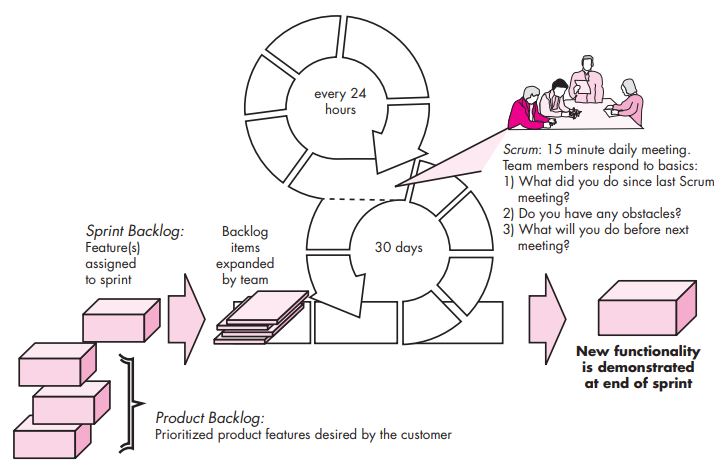
\includegraphics[width=0.85\textwidth]{scrum.png}
        \end{center}
    \label{scrumFlow}
    \legend{Fonte: \cite{pressman}}
\end{figure}

\subsection{Kanban}
\label{fundSWKanban}

O Kanban\footnote{A palavra é originária do mandarim e, em português, significa painel de controle.} torna-se cada vez mais uma maneira popular de visualizar e limitar o trabalho em andamento no desenvolvimento de \textit{softwares}. Além disso, sua utilização em processos existentes cataliza mudanças culturais e oferece agilidade nos negócios \cite{kanbanBook}.

Dessa forma, seguindo os preceitos do manifesto ágil, o \textit{framework} Kanban fornece um sistema de gerenciamento de processo visual que auxilia na tomada de decisões sobre o que, quando e quanto produzir \cite{kanbanBook2}. Embora não seja obrigatório, a visualização do fluxo do processo com Kanban geralmente é feita através de um Kanban \textit{board} (quadro Kanban). Este quadro, de caráter simples, apresenta um processo em fluxo da esquerda para a direita, onde as colunas representam a divisão de etapas deste e cada cartão, uma atividade a ser realizada. Em Engenharia de \textit{software}, geralmente, cada coluna representa uma etapa do desenvolvimento e o cartão, uma funcionalidade a ser implementada no sistema. A Figura \ref{kanbanFlow} apresenta um exemplo de quadro Kanban.

\begin{figure}[ht]
    \caption{Fluxo do processo de desenvolvimento no Kanban.}
       	\begin{center}
            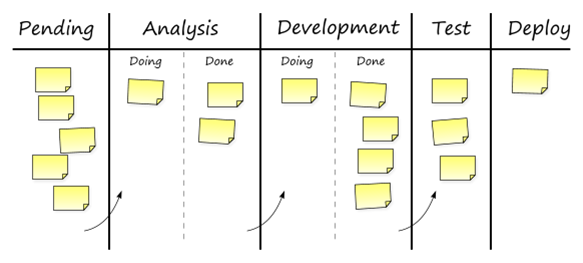
\includegraphics[width=0.8\textwidth]{kanban.png}
        \end{center}
    \label{kanbanFlow}
    \legend{Fonte: \url{https://bobsleanlearning.wordpress.com/2010/07/28/kanban-distilled/}, Acessado em novembro de 2018.}
\end{figure}

Portanto, não é incomum no processo de desenvolvimento de sistemas, a combinação da metologia Scrum aliada ao Kanban. Assim, é possível usufruir do desenvolvimento ágil de maneira organizada, tornando capaz o entendimento geral dos processos (e como eles se comunicam) por parte dos \textit{stalkeholders}, isto é, as pessoas envolvidas neste, através do quadro Kanban durante as \textit{Sprints} e ao longo de todas as etapas de implementação do sistema.

\subsection{Considerações finais}
\label{fundConsideracoes}

Neste capítulo foram apresentados conceitos importantes que permearam todo o desenvolvimento do protótipo da rede social Portal de Vagas. A análise das diferentes arquiteturas de \textit{software} -em especial, cliente-servidor, centrada em dados e MVC- auxiliou na tomada de decisões ainda na etapa de projeto de sistema, visto que, ao adotar diferentes modelos de arquitetura, podemos basear o desenvolvimento do \textit{software} em regras e conceitos já bem definidos e testados ao longo de anos, aumentando a qualidade do produto final. Vimos também tópicos referentes à modelagem de banco de dados porque, há um bom tempo, sistemas presentes na Internet que utilizam SGBDs para armazenar e manipular dados são bastante comuns. Contudo, similar às decisões de arquitetura, decisões de banco de dados são cruciais ao desenvolver uma aplicação escalável; portanto, a utilização de regras e técnicas para aumentar a manutenção e performance do SGBD são essenciais. Por fim, foram apresentados processos de desenvolvimento de \textit{software} aplicados neste trabalho, como a metologia ágil e seus \textit{frameworks} complementares: Scrum e Kanban.